\section{Setup}
\label{sec:setup}
\subsection{Data and the label error}
Waterbirds has 4,795 training, 1,199 validation and 5,794 test images. A group is a pair (bird class, background); the test groups landbird-on-land, landbird-on-water, waterbird-on-land and waterbird-on-water contain 2,255, 2,255, 642 and 642 images. WGA is the minimum of the four group accuracies, computed per backbone and then averaged.

The generating script \cite{sagawa2020code} labels a CUB species as a waterbird if its lower-cased name contains any keyword from a list of seabirds and waterfowl, one of which is \texttt{tern}. The substring also occurs in \texttt{eastern} and \texttt{western}. Three species match no intended keyword and are labelled waterbird only through this match: 021 Eastern Towhee, 088 Western Meadowlark and 102 Western Wood-Pewee. Western Grebe and Western Gull also contain \texttt{tern} but are waterbirds through \texttt{grebe} and \texttt{gull}; a pass over all 46 waterbird-labelled species finds no other case. The affected images are 72 training, 18 validation (11 of the 133 waterbird-on-land and 7 of the 133 waterbird-on-water images) and 90 test images (43 and 47 of the two waterbird test groups of 642).

We use three label sets. \emph{Official} is the released metadata. \emph{Corrected} relabels the affected images as landbirds, which also moves them to the landbird groups. For fitting we also consider \emph{drop}, which removes the 18 affected validation images. Backbones are always trained on the official training labels.

\subsection{Backbones and heads}
We use seven ResNet-50 backbones saved from earlier runs: five standard ERM backbones (seeds 0--4, 100 epochs) and two ERM$^*$ backbones (seeds 0--1, 400 epochs with augmentation), reported separately because they are different recipes. All heads act on frozen 2,048-dimensional features of the validation and test images.

\textbf{DPE.} Fifteen two-prototype distance-based heads are trained in sequence on group-balanced subsets of the validation features \cite{to2025dpe}: 20 epochs per head, batch size 256, learning rate $10^{-3}$, momentum 0.9, entropic scale 30, covariance penalty $5\times10^5$ (decaying by stage for standard ERM, constant for ERM$^*$ as in the preserved recipes). For standard ERM each head keeps the epoch with the highest WGA on its own training pool. The prediction averages the head probabilities. \emph{Full-validation DPE}, fitted on all 1,199 images, is the reference throughout.

\textbf{DFR-lite.} As a second validation-label method we fit group-weighted L1-penalised logistic regression on standardised features of the validation set, choosing $C\in\{0.01,0.03,0.1,0.3,1\}$ by five-fold validation WGA. It follows DFR \cite{kirichenko2023dfr} in using the same frozen features and group labels, but without DFR's repeated balanced subsampling.

\subsection{Protocols}
\textbf{Label study.} Full-validation DPE (five head seeds per backbone) and DFR-lite are refitted on the official, corrected and drop validation sets, and every model is scored on official and corrected test labels. With official labels and head seed 0, the refit reproduces the saved ensembles exactly.

\textbf{Spending the validation set.} We compare full-validation DPE with three ways of adding a step on top of it.
\begin{itemize}
\item \emph{Held-out combiners}: heads on 720 images and a combiner on the other 479 (an affine map of the ensemble score, a linear residual on head disagreements, or a dropout MLP), against the matched 720-image ensemble and against full-validation DPE.
\item \emph{Cross-fitting}: five 15-head ensembles, each trained on four fifths of the validation set; one affine map $\sigma(a s+b)$ of the score $s=\mathrm{logit}\,\bar q$ is fitted on the 1,199 out-of-fold scores and applied to each fold ensemble before averaging, so no image is held back from head training.
\item \emph{Controls}: the uncalibrated fold ensemble; the same pipeline with $a=1$ (offset only); the offset or threshold learnt on the out-of-fold scores and transferred to full-validation DPE; and a 75-head bag of five full-validation ensembles, which has as many heads as cross-fitting but no held-out scores.
\end{itemize}
Calibrators minimise group-averaged or worst-group cross-entropy with penalty $\lambda[(a-1)^2+b^2]$, $\lambda\in\{0.01,0.1\}$, using 400 full-batch Adam steps.

\textbf{Validation-only selection.} The calibration setting is chosen by the lowest group-balanced negative log-likelihood (primary) or the highest WGA (secondary) in an inner five-fold cross-validation on the out-of-fold scores; heads are not refitted inside it. The whole procedure, including the head-training seeds and the fold and 720/479 splits, is repeated for ten split seeds, and full-validation DPE is retrained with the same seeds, so every comparison is paired within a cell.

\textbf{Statistics.} Differences are paired per backbone, averaged over seeds within a backbone, and reported with pointwise 95\% $t$ intervals over the five standard-ERM backbones. With two ERM$^*$ backbones we report means only. Seeds and splits are repeats within a backbone and are not counted as independent evidence.

\section{Results}
\label{sec:results}
\subsection{Reproduction}
Table~\ref{tab:repro} compares our full-validation DPE with the published numbers. Our standard-ERM DPE is 1.1--1.4\pp{} below the reported 91.0\%; ERM$^*$ matches. To check whether the gap comes from our implementation, we ran the authors' code end to end on two fresh ERM backbones. The backbones match the reported ERM accuracy (69.3\% against 69.1\%), and DPE reaches 89.4\% and 86.5\%. The official pipeline is therefore also below 91.0\% in our hands, and our results should be read relative to our own full-validation DPE. Over ten head seeds the WGA of full-validation DPE has a within-backbone SD of 0.40\pp{} (standard ERM) and 0.33\pp{} (ERM$^*$), which sets the scale for the differences below.

\begin{table}[t]
\centering\small
\caption{Reproduction of full-validation DPE (test WGA, \%, official labels).}
\label{tab:repro}
\begin{tabular}{@{}llrr@{}}
\toprule
Recipe & Run & DPE & Reported \cite{to2025dpe}\\\midrule
ERM & ours, 5 backbones, saved heads & 89.60 & 91.0\\
ERM & ours, 5 backbones, mean over 10 head seeds & 89.88 & 91.0\\
ERM & authors' code, fresh backbones (seeds 5, 6) & 89.41, 86.47 & 91.0\\
ERM$^*$ & ours, 2 backbones, saved heads & 94.08 & 94.1\\
ERM$^*$ & ours, 2 backbones, mean over 10 head seeds & 93.88 & 94.1\\
\bottomrule
\end{tabular}
\end{table}

\subsection{The label error dominates DPE's worst group}
Waterbird-on-land is the worst group of full-validation DPE on every backbone. Table~\ref{tab:errors} counts its test errors. On standard ERM, 37--39 of the 43 mislabelled images in this group are predicted landbird, which is correct, and are counted as errors; they make up 55--62\% of the group's errors. On ERM$^*$ the share is about half.

\begin{table}[t]
\centering\small
\caption{Errors of full-validation DPE (saved heads) in the waterbird-on-land test group (642 images, 43 of them from the three mislabelled species).}
\label{tab:errors}
\resizebox{\linewidth}{!}{\begin{tabular}{@{}lrrrrrrr@{}}
\toprule
& \multicolumn{5}{c}{Standard ERM backbone} & \multicolumn{2}{c}{ERM$^*$}\\
& 0 & 1 & 2 & 3 & 4 & 0 & 1\\\midrule
Official WGA (\%) & 89.56 & 90.65 & 89.10 & 89.25 & 89.41 & 94.39 & 93.77\\
Errors in waterbird-on-land & 67 & 60 & 70 & 69 & 68 & 36 & 40\\
\quad of which mislabelled species & 37 & 37 & 39 & 38 & 39 & 18 & 21\\
\bottomrule
\end{tabular}}
\end{table}

\subsection{Cleaning 18 validation labels}
Table~\ref{tab:labels} gives the main result. Refitting DPE on corrected validation labels raises WGA on corrected test labels by $+2.48$\pp{} ($[+1.80,+3.15]$, positive on all five standard-ERM backbones); dropping the 18 images instead gives $+2.46$\pp{} ($[+1.90,+3.01]$). On ERM$^*$ the gains are $+2.12$ and $+2.08$\pp. The effect is larger than every aggregation effect in Section~\ref{sec:spend}, including settings chosen after looking at test results, and about six times the head-seed SD. DFR-lite also gains on standard ERM ($+1.56$\pp, $[+1.19,+1.94]$) but not on ERM$^*$.

Scored with the official test labels, the same fix looks harmful: $-0.83$\pp{} ($[-1.34,-0.31]$) for DPE and $-1.92$\pp{} for DFR-lite. The refitted models predict landbird for more of the 90 mislabelled test images (on average 86 instead of 78 for DPE on standard ERM), which the official labels count as errors. A method that learns the correct concept is therefore penalised by the benchmark, and an improvement in label quality is invisible, or even negative, in results reported on the official labels.

\begin{table}[t]
\centering\small
\caption{Test WGA (\%) after fitting on official, corrected or reduced (drop) validation labels, scored on official and corrected test labels. Means over five head seeds (DPE) and over backbones. $\Delta$: paired difference to the official-label fit on corrected test labels, with 95\% interval over the five standard-ERM backbones.}
\label{tab:labels}
\resizebox{\linewidth}{!}{\begin{tabular}{@{}llrrrrr@{}}
\toprule
& & \multicolumn{3}{c}{Standard ERM ($n=5$)} & \multicolumn{2}{c}{ERM$^*$ ($n=2$)}\\
Method & Fit labels & Official & Corrected & $\Delta$ corrected & Official & Corrected\\\midrule
DPE & official & 89.89 & 90.34 & -- & 93.88 & 93.45\\
DPE & corrected & 89.07 & \textbf{92.81} & $+2.48$ $[+1.80,+3.15]$ & 92.74 & \textbf{95.57}\\
DPE & drop & 89.07 & 92.79 & $+2.46$ $[+1.90,+3.01]$ & 93.16 & 95.53\\\midrule
DFR-lite & official & 88.62 & 88.97 & -- & 92.68 & 94.18\\
DFR-lite & corrected & 86.70 & 90.53 & $+1.56$ $[+1.19,+1.94]$ & 88.94 & 94.13\\
DFR-lite & drop & 86.54 & 90.42 & $+1.45$ $[+1.07,+1.83]$ & 89.25 & 94.16\\
\bottomrule
\end{tabular}}
\end{table}

\subsection{Spending the validation set}
\label{sec:spend}
\textbf{Held-out combiners.} With fixed settings, an affine map fitted on the 479 reserved images improves on the matched 720-image ensemble in all six combinations of recipe and partition, which is the comparison a combiner is usually reported against. Against full-validation DPE the picture changes (Fig.~\ref{fig:allocation}): a linear residual is ahead by $+0.75$, $+0.93$ and $+0.67$\pp{} on standard ERM but behind by $-0.42$, $-0.37$ and $-1.17$\pp{} on ERM$^*$, and the dropout MLP ranges from $-1.22$ to $+0.81$\pp{} across the six combinations. When the setting is chosen on validation data (Table~\ref{tab:spend}), the linear residual is $-0.86$\pp{} and the affine combiner $-0.05$\pp{} relative to full-validation DPE.

\begin{figure}[t]
\centering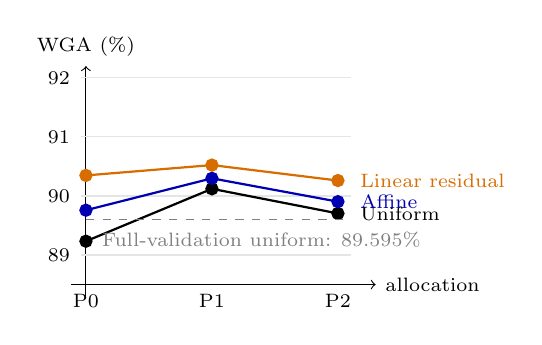
\begin{tikzpicture}[x=1.6cm,y=0.75cm,font=\scriptsize]
\draw[->] (-0.12,0) -- (2.3,0) node[right]{allocation};
\draw[->] (0,-0.2) -- (0,3.7) node[above]{WGA (\%)};
\draw[gray!20] (-0.04,0.5) -- (2.1,0.5);
\node[left] at (-0.05,0.5) {89};
\draw[gray!20] (-0.04,1.5) -- (2.1,1.5);
\node[left] at (-0.05,1.5) {90};
\draw[gray!20] (-0.04,2.5) -- (2.1,2.5);
\node[left] at (-0.05,2.5) {91};
\draw[gray!20] (-0.04,3.5) -- (2.1,3.5);
\node[left] at (-0.05,3.5) {92};
\node[below] at (0,0) {P0};
\node[below] at (1,0) {P1};
\node[below] at (2,0) {P2};
\draw[thick,black] plot[mark=*] coordinates {(0,0.73373) (1,1.62131) (2,1.20439)};
\node[right,black] at (2.1,1.20439) {Uniform};
\draw[thick,blue!70!black] plot[mark=*] coordinates {(0,1.25881) (1,1.79862) (2,1.40383)};
\node[right,blue!70!black] at (2.1,1.40383) {Affine};
\draw[thick,orange!85!black] plot[mark=*] coordinates {(0,1.84780) (1,2.02310) (2,1.76106)};
\node[right,orange!85!black] at (2.1,1.76106) {Linear residual};
\draw[dashed,gray] (0,1.095) -- (2.05,1.095);
\node[gray,anchor=west] at (0.05,0.75) {Full-validation uniform: 89.595\%};
\end{tikzpicture}
\caption{Standard-ERM mean WGA of three fixed procedures at three 720/479 partitions (affine and linear residual: average loss, $\lambda=0.1$). Dashed: full-validation DPE. Saved heads, split seed 0.}
\label{fig:allocation}
\end{figure}

\textbf{Cross-fitting and recalibration.} Table~\ref{tab:spend} summarises the ten-split-seed study. With validation-only selection, cross-fitted affine recalibration is $-0.17$\pp{} ($[-0.33,-0.02]$, no backbone positive) with the primary rule and $-0.08$\pp{} with the secondary rule. The likelihood rule chose the weakest regularisation in all 70 cells. Even the setting we had highlighted earlier after looking at test results (average loss, $\lambda=0.1$), which gave $+0.47$\pp{} on split seed 0, averages $+0.17$\pp{} over ten split seeds, and the full-validation DPE of split seed 0 happened to be 0.28\pp{} below its ten-seed mean. Cross-fitting without recalibration is level with a 75-head bag ($+0.07$\pp, $[-0.32,+0.46]$), so what remains of its gain is explained by having more heads.

\begin{table}[t]
\centering\small
\caption{Spending the validation set: test WGA difference (pp, official labels) against full-validation DPE retrained with the same seeds, averaged over ten split seeds. Interval: 95\% over five standard-ERM backbones.}
\label{tab:spend}
\begin{tabular}{@{}lrrr@{}}
\toprule
& \multicolumn{2}{c}{Standard ERM} & ERM$^*$\\
Procedure & $\Delta$ & 95\% interval & $\Delta$\\\midrule
Full-validation DPE (WGA, \%) & 89.88 & & 93.88\\\midrule
75-head bag (five full-validation ensembles) & $+0.06$ & $[-0.08,+0.20]$ & $+0.17$\\
Cross-fit, uniform & $+0.13$ & $[-0.28,+0.53]$ & $+0.18$\\
Cross-fit, affine, fixed setting & $+0.17$ & $[-0.01,+0.34]$ & $+0.11$\\
Cross-fit, offset only ($a=1$), fixed setting & $+0.17$ & $[-0.01,+0.34]$ & $+0.11$\\
Cross-fit, affine, selected (NLL) & $-0.17$ & $[-0.33,-0.02]$ & $-0.08$\\
Cross-fit, affine, selected (WGA) & $-0.08$ & $[-0.17,+0.01]$ & $+0.03$\\
Full DPE, offset transferred from folds & $-0.57$ & $[-0.76,-0.39]$ & $-0.49$\\
720/479, affine, selected (NLL) & $-0.05$ & $[-0.17,+0.06]$ & $-0.24$\\
720/479, linear residual, selected (NLL) & $-0.86$ & $[-1.32,-0.39]$ & $-0.76$\\
DFR-lite & $-1.51$ & $[-1.83,-1.20]$ & $-1.28$\\
\bottomrule
\end{tabular}
\end{table}

\textbf{Recalibration is a threshold shift.} Cross-fitted affine recalibration and the offset-only control have the same mean WGA at the fixed setting and differ by at most 0.09\pp{} at the other three settings. On split seed 0 they have identical accuracy in all four groups on all seven backbones at the fixed setting. The fitted slopes are 1.20--1.31 and the offsets at most 0.011 in absolute value, while the median absolute test logit of DPE is only 0.10--0.16, so the map moves the decision boundary by a few thousandths and the slope has no measurable effect. Thresholds learnt on the out-of-fold scores do not transfer: applied to full-validation DPE, which is trained on 25\% more images, they lower WGA on every standard-ERM backbone ($-0.57$\pp).

\subsection{Label errors change method comparisons}
Re-scoring the split-seed-0 models on corrected test labels changes the comparison between methods. The uniform fold ensemble is $+0.54$\pp{} ahead of full-validation DPE on official labels and $-0.18$\pp{} behind on corrected labels (per backbone $+0.91$, $-0.78$, $+0.43$, $-2.43$, $+0.96$); the affine variant moves from $+0.47$ to $+0.64$\pp. Differences of half a point between Waterbirds methods can therefore depend on whether the 90 mislabelled test images are corrected, and on how a method happens to treat these species.

\section{Discussion and Limitations}
\textbf{What limits validation-label methods.} For DPE on Waterbirds, the quality of 18 validation labels matters more than every scheme we tried for spending the validation set. The mechanism is plausible: DPE trains each head on a group-balanced subset, so the 11 mislabelled waterbird-on-land images are drawn into the minority group at a much higher rate than their share of the data, and they teach the heads that these landbirds are waterbirds. The official test labels then reward that mistake on the 43 matching test images. We recommend that methods trained on Waterbirds validation labels report results on corrected labels alongside the official ones, and fit on corrected validation labels.

\textbf{Limitations.} The study covers one dataset and seven backbones from two recipes, with only two ERM$^*$ backbones. The backbones and test set were inspected during earlier development, and the label error was first noticed in test errors; the correction itself is defined by the generator code and does not use any model. Backbones were trained on the official training labels, which include 72 affected images; retraining them could change the size of the effect. We correct only these three species; other issues, such as images that show several birds \cite{asgari2022masktune}, remain. Our standard-ERM DPE is below the published figure, as is the authors' code in our hands. Intervals are pointwise and over backbones only. Improved WGA does not show that a model relies less on backgrounds.

\section{Conclusion}
Methods that train a light head on the Waterbirds validation set inherit a known but unmeasured label error: three landbird species are labelled waterbird because ``tern'' is a substring of ``Eastern'' and ``Western''. For diverse prototypical ensembles, these species account for half or more of the errors in the worst group, and fixing the 18 affected validation labels improves worst-group accuracy on corrected labels by about 2.5\pp{} on every standard-ERM backbone, while the official labels score the fix as a loss. Spending the same validation set through cross-fitting, recalibration or learned combiners does not beat DPE fitted on all images once settings are chosen on validation data, and recalibration reduces to a threshold shift. Cleaning labels, not allocating them, is the larger lever for this family of methods, and benchmark comparisons at the scale of half a point should report corrected labels.
